\section{弾性による影響}

粘性による影響では説明が十分にできない
球の落下によって生じる応力$\tau_\text{U}$に関して,
\begin{eqnarray}
    \tau_U \sim k \times \left(\frac{U_\text{T}}{a}\right),
    \label{eq:tauU}
\end{eqnarray}
といった式で近似できる.この式(\ref{eq:tauU})を用いて,
応力比
Fig.\ref{fig:elastcity}に示す.

\begin{figure}[h]
    \centering
    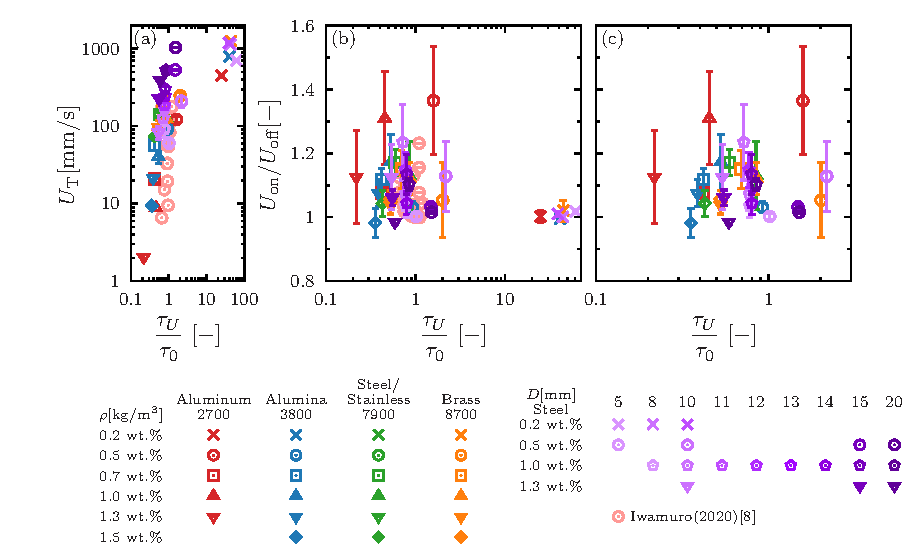
\includegraphics[width=1.0\textwidth]{5-Results/elastcity.eps}
    \caption{Relationship between velocity ratio and elasticity ratio$\tau_\text{U}/\tau_\text{0}$.}
    \label{fig:elastcity}
\end{figure}
